\section{Research Design}
\label{sec:researchdesing}

The motivation to write this paper comes from experiences on teaching. During the classes of Distributed Systems and Parallel Programming, a graduate course at University of São Paulo...

\begin{description}
\item[RQ1:] \textit{Which API is easier to learn and use according to the student perceptions?}
%
...
\item[RQ2:] \textit{Which API is better to improve the performance according to the student perceptions?}
%
...

\end{description}

\subsection{Student Background}

\begin{figure}[htpb]
    \centering
    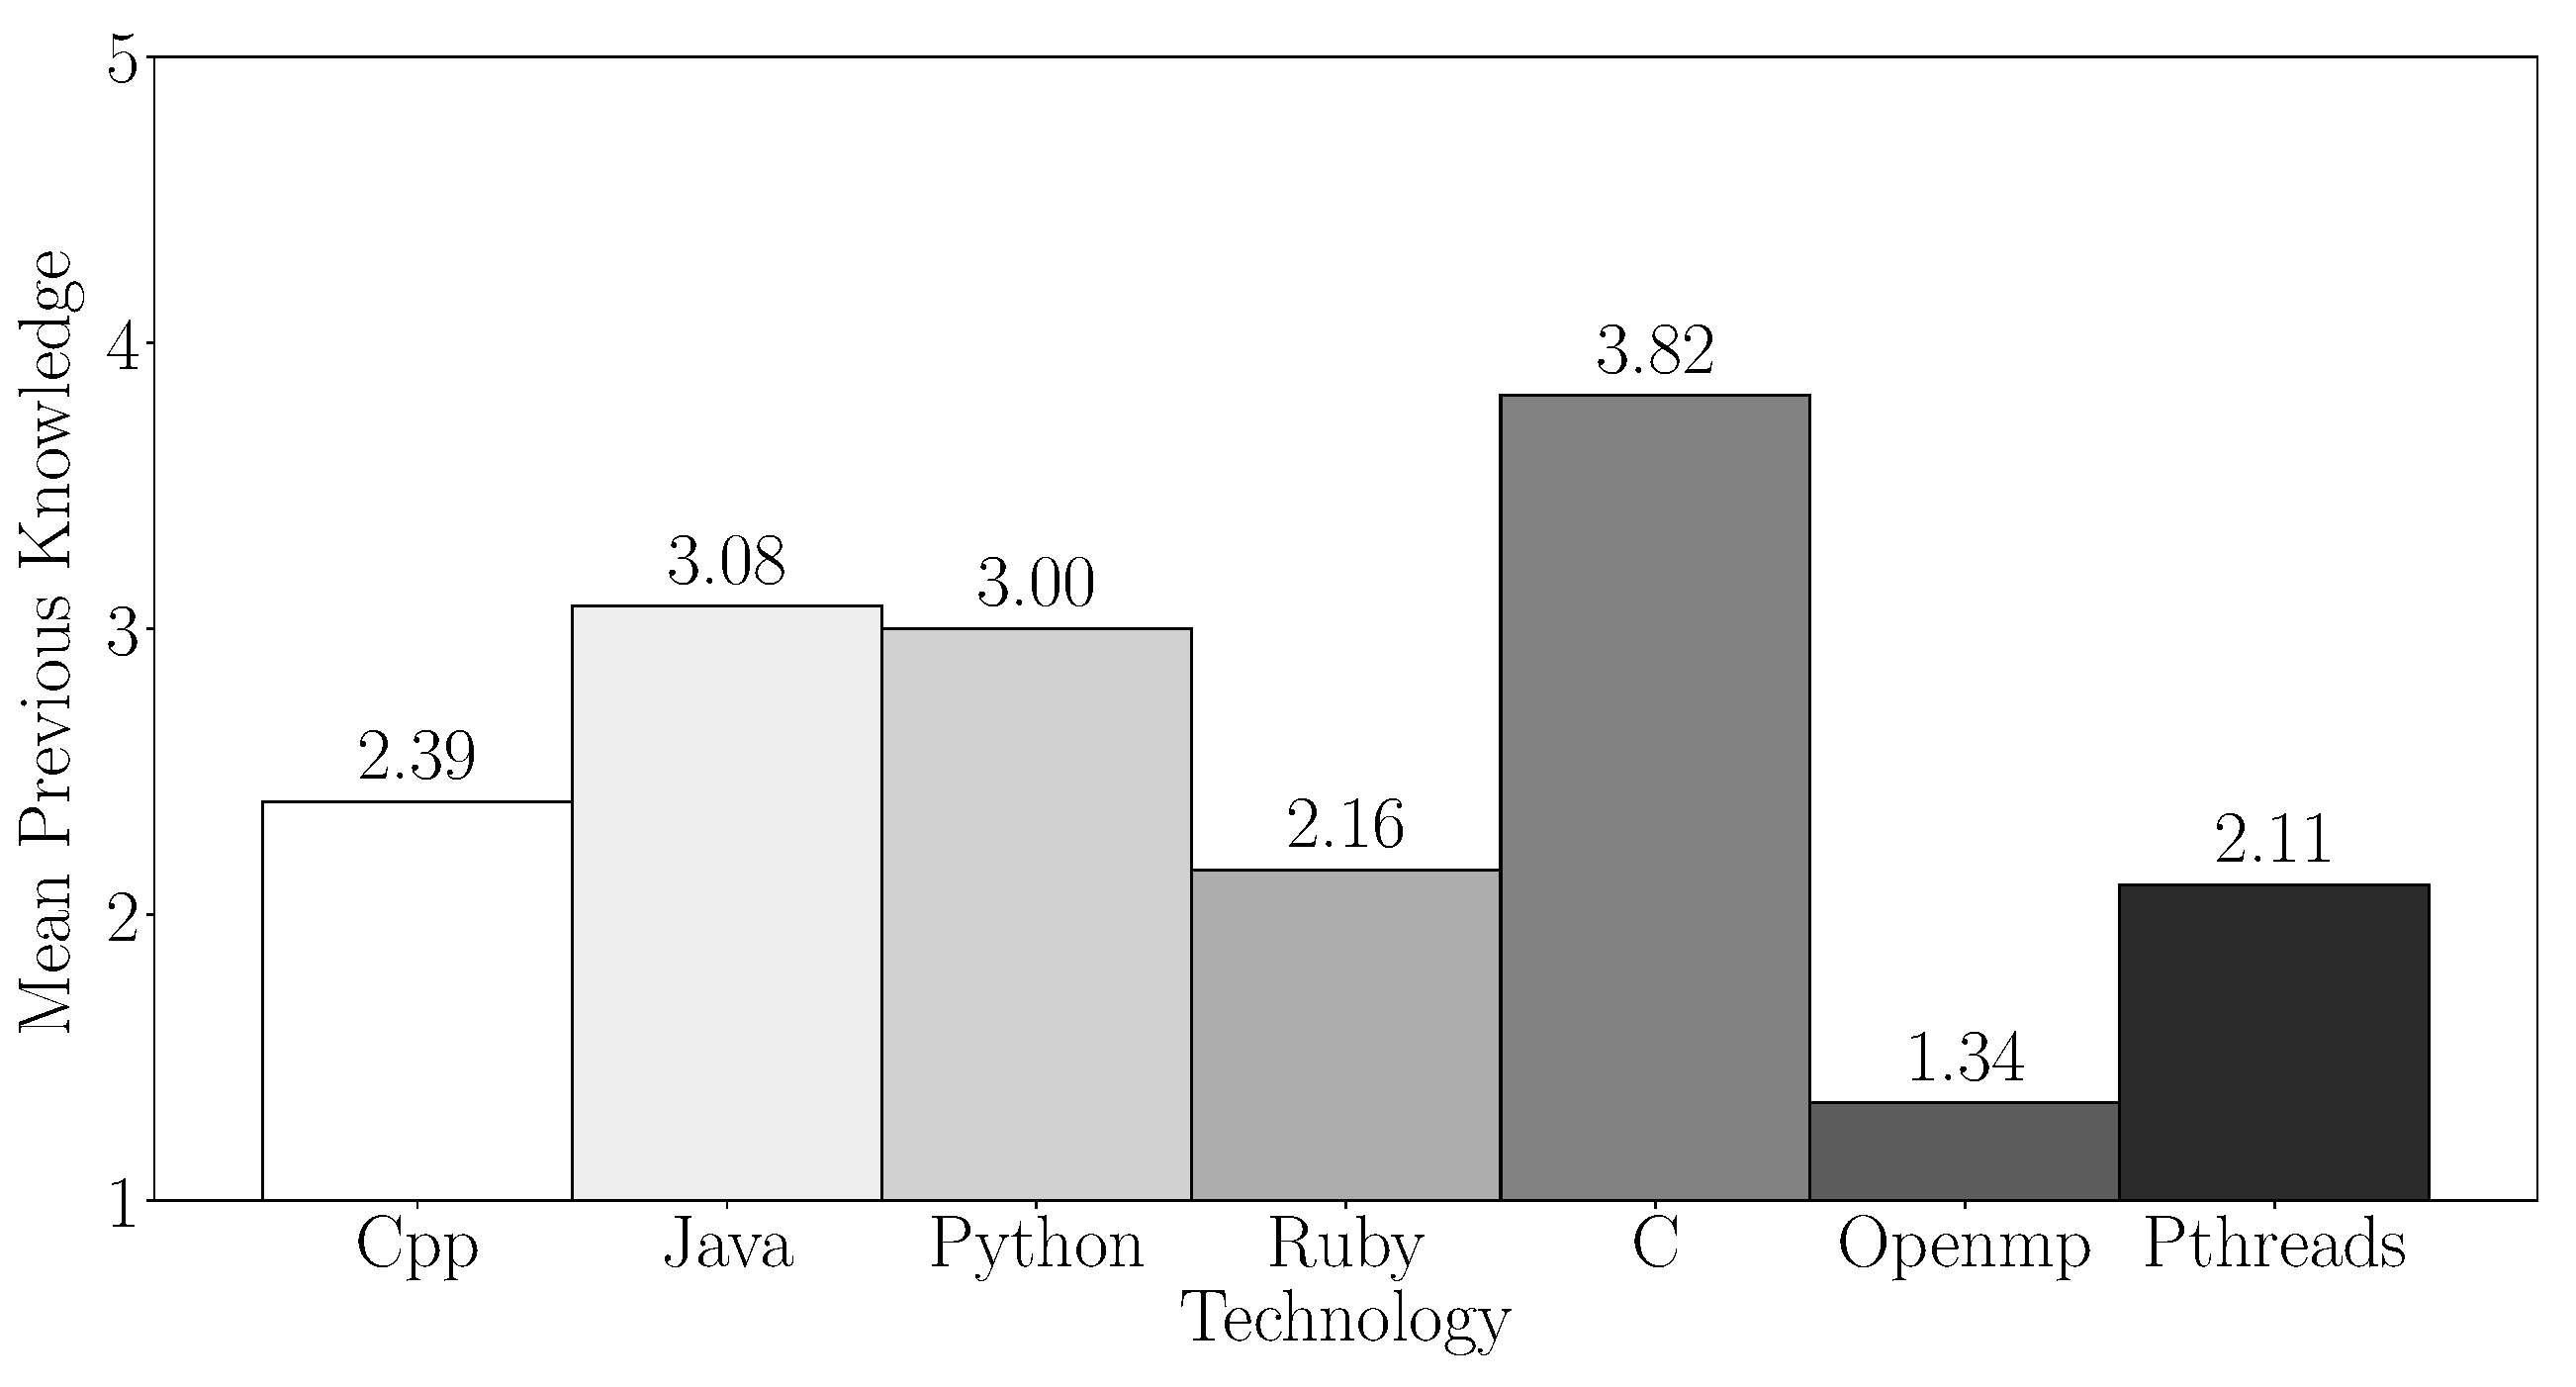
\includegraphics[width=0.85\columnwidth]{background_mean_knowledge}
    \caption{Student mean knowledge \textit{before} the assignment}
    \label{fig:student-mean-knowledge}
\end{figure}

\begin{figure}[htpb]
    \centering
    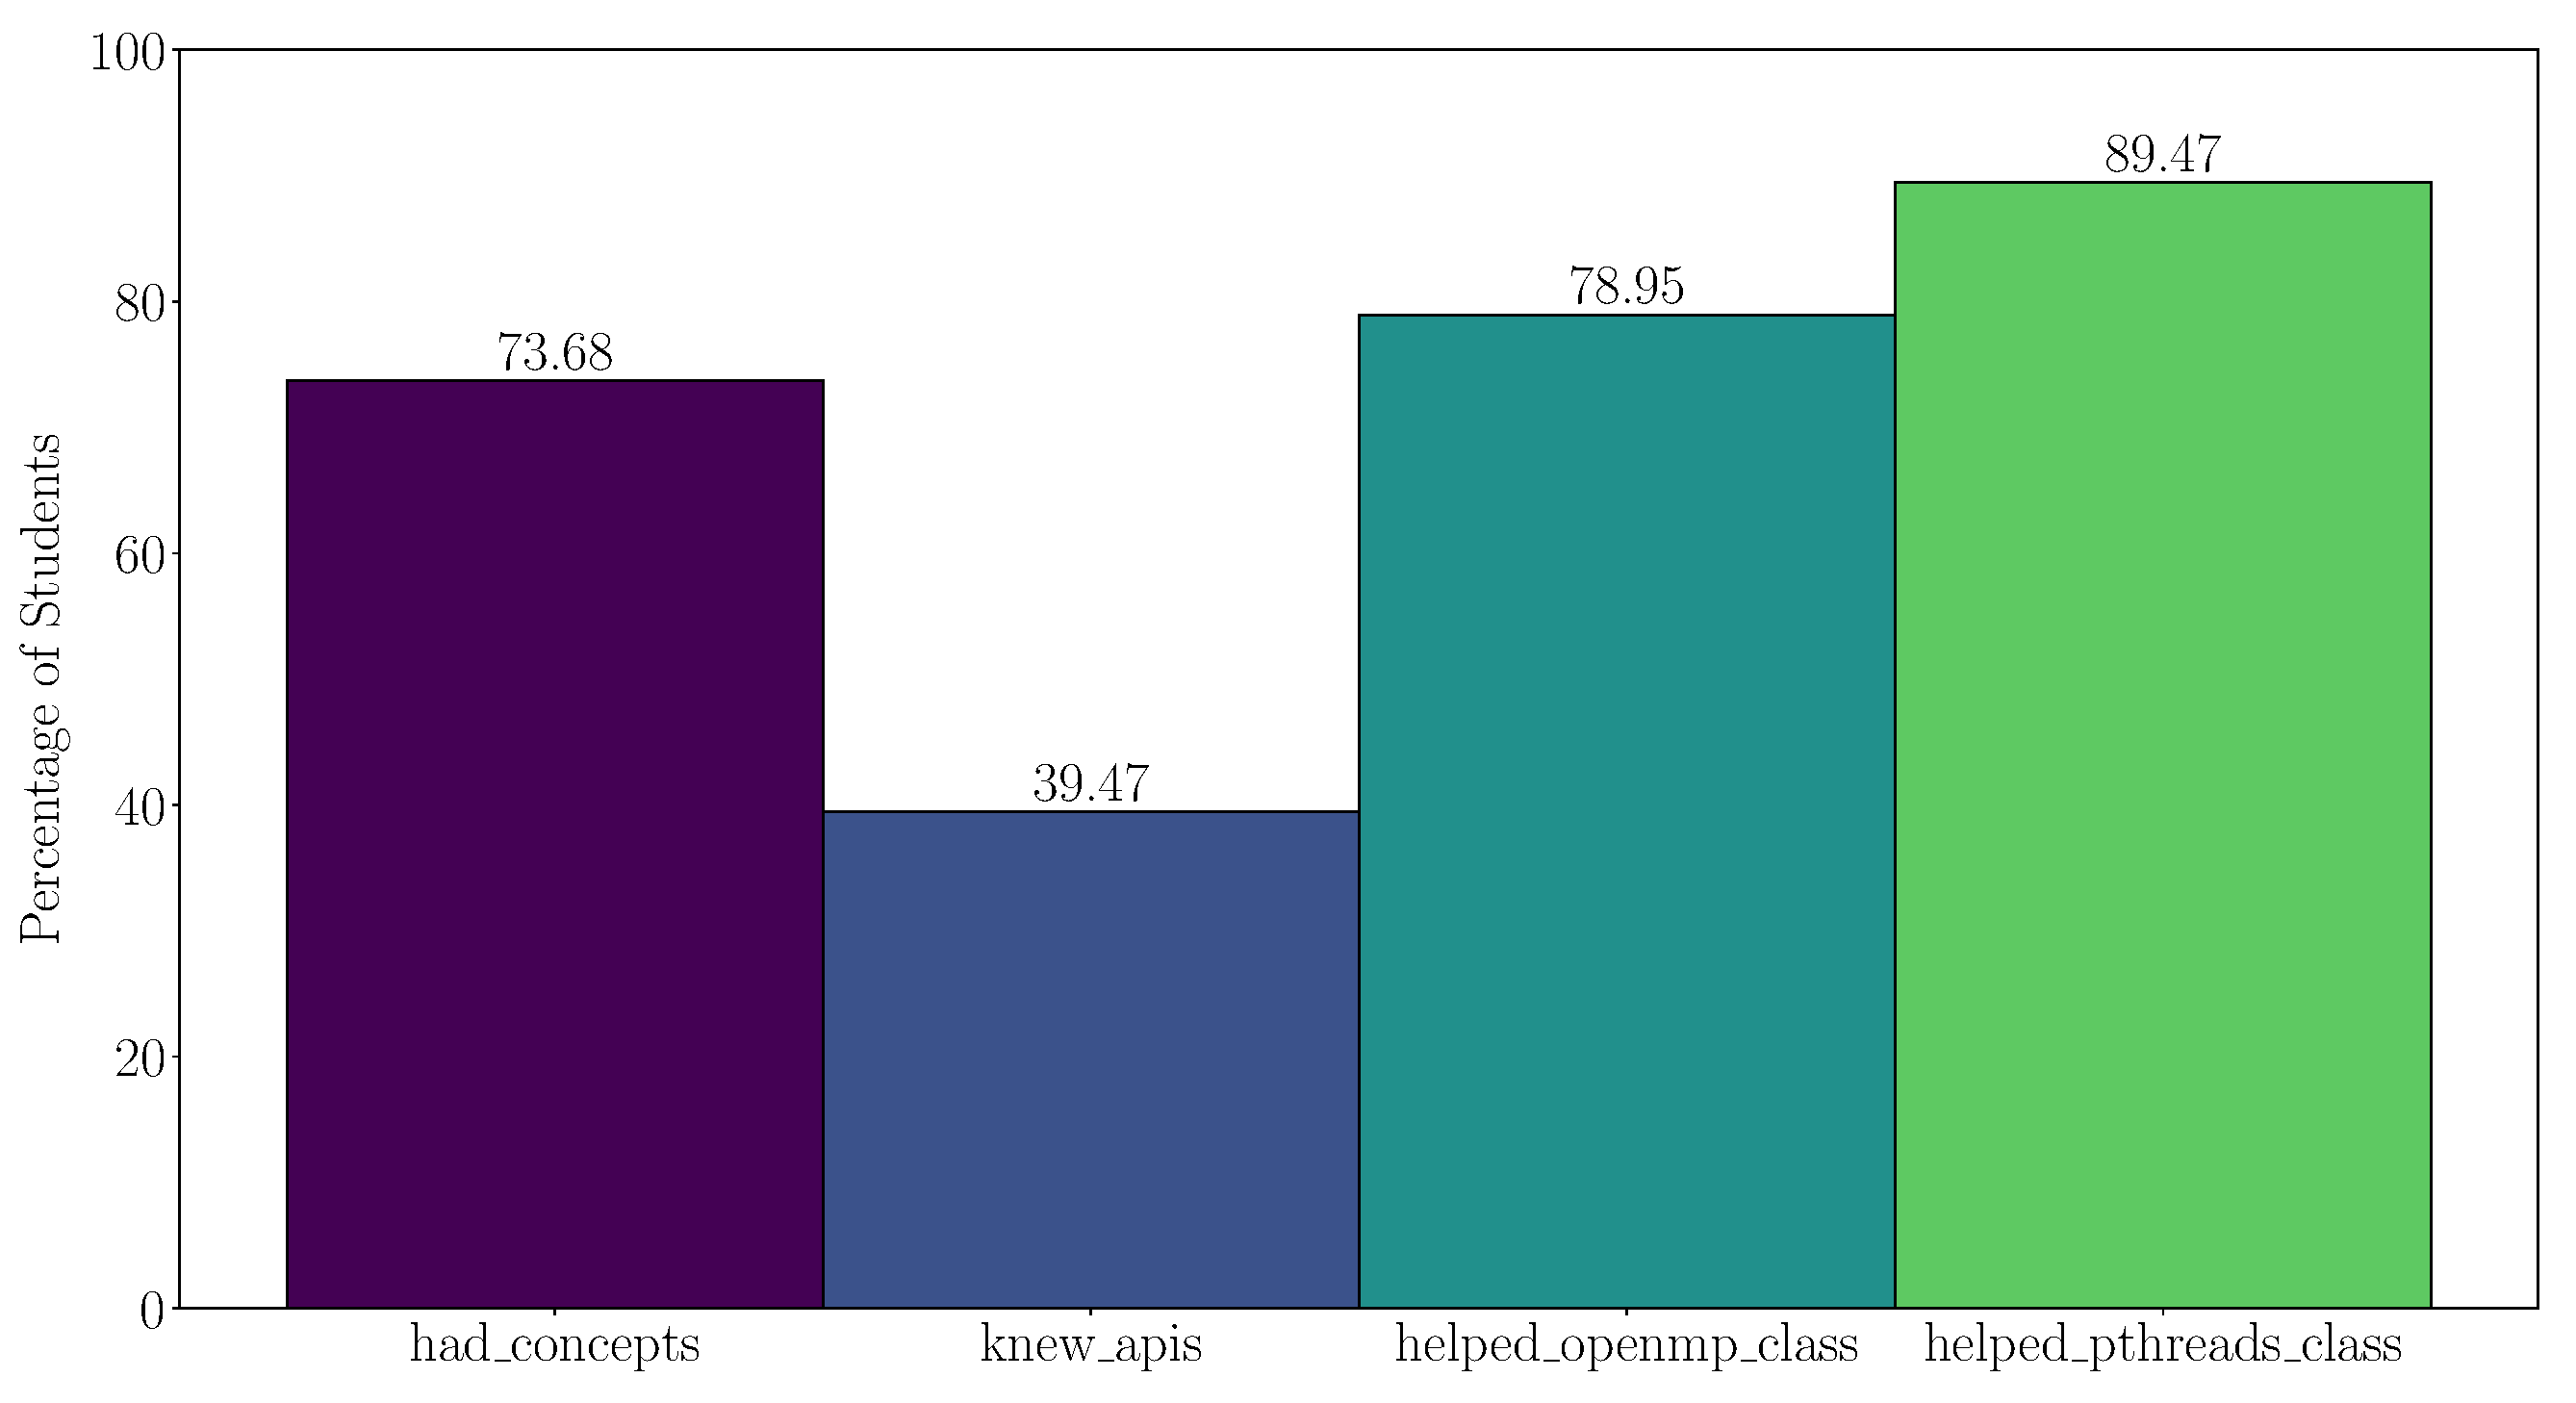
\includegraphics[width=0.85\columnwidth]{yes_no_questions}
    \caption{Student API knowledge \textit{before} the assignment and their relation to classes}
    \label{fig:student-knowledge-yes-no}
\end{figure}


